\documentclass[10pt]{scrartcl}
\usepackage[utf8]{inputenc}
\usepackage{graphicx}
\usepackage{wrapfig}
\usepackage{hhline}
\author{Dane Wicki}
\title{Universal data acquisition}
\subtitle{FS17 Praxismodul}
\renewcommand{\contentsname}{Inhaltsverzeichnis}
\begin{document}
\maketitle
\tableofcontents
\section{Einleitung, Problembeschreibung}
\subsection{Gescheftsfeld der Firma}
Die Siemens AG ist ein führender internationaler Technologiekonzern, der seit mehr als 165 Jahren für technische Leistungsfähigkeit, Innovation, Qualität, Zuverlässigkeit und Internationalität steht. Das Unternehmen ist in mehr als 200 Ländern aktiv, und zwar schwerpunktmäßig auf den Gebieten Elektrifizierung, Automatisierung und Digitalisierung. Siemens ist weltweit einer der größten Hersteller energieeffizienter ressourcenschonender Technologien. Das Unternehmen ist einer der führenden Anbieter effizienter Energieerzeugungs- und Energieübertragungslösungen, Pionier bei Infrastrukturlösungen sowie bei Automatisierungs-, Antriebs- und Softwarelösungen für die Industrie. Darüber hinaus ist das Unternehmen ein führender Anbieter bildgebender medizinischer Geräte wie Computertomographen und Magnetresonanztomographen sowie in der Labordiagnostik und klinischer IT.
\subsection{Projektkontext}
Die Firma Siemens BT in Zug ist zuständig für die Entwicklung von Brandmeldern.
Um die Qualität der Brandmelder zu gewährleisten, werden diese unter Zuhilfenahme
verschiedener Apparaturen und Testaufbauten getestet. Dies geschieht bei vielen Aufbauten automatisch und mit konsistenter Aufzeichnung der Daten, welche der Melder und etwaige Referenz-Geräte erzeugen. Es gibt jedoch weiterhin aufbauten, bei welchen die Aufzeichnung weder Automatisch noch Konsistent gespeichert werden kann oder nur unter grossen Anstrengungen der Arbeitenden. Diesen Zustand gilt es nun zu verbessern.
Dazu soll eine Software entwickelt werden, die aus verschiedenen Ressourcen (verschiedenen
Datenquellen) die Daten sammelt und diese in eine auswertbare Excel-Datei exportiert. Dies
Software basiert auf einer bestehenden Software, welche für das Brandlabor entwickelt wurde.
Es sollen dabei Bestandteile dieser Bestehenden Software verwendet werden.
\subsection{Problembeschreibung}
\subsection{Projektziele}
.Bei vielen kleinen Aufbauten ist keine Software vorhanden ist, oder nur teilweise vorhanden, welche die zu sammelnden Daten zusammenträgt. Dieser mangel an Software führt dazu, dass nur auf umständliche art und weise getestet werden kann. Dies stellt eines der Probleme dar. Dieser Umstand führt auf einen erhöhten Zeitaufwand bei einem Testdurchlauf, da alle Daten manuell zusammengetragen werden müssen. Zudem kommt bei manchen Aufbauten dazu, dass sie selten gebraucht werden. Der fehlende Zyklische Gebrauch jener Aufbauten führt zu einer erhöhten Einarbeitungsperiode. Diese Einarbeitungsperiode sowie der Erhöte Zeitaufwand für einen Testdurchlauf soll durch eine vereinheitlichung beseitigt werden. Dazu soll die Software an möglichst allen Aufbauten eingesetzt werden können, welche keine eigene Spezielle Software besitzten.

Hinzu kommt eine anpassung eines UL-Standardes für einen bestehenden Brandmelder. Dieser neue Standard führte dazu, dass die Testabteilung der Siemens einen neuen Testaufbau bestellte. Im Rahmen der Bestellung wurde jedoch nur die Apparatur zum Testen bestellt, keine Passende Software, welche alle Daten während eines Testlaufes aufzeichnen könnte. Ziel ist es die Software mit ankuft der Apparatur in Betrieb zu nehmen.
\section{Projektergebnisse}
\subsection{Ergebnisse}
Die folgenden Ergebnisse müssen im Rahmen dieses Projektes erarbeitet werden:
\begin{itemize}
	\item DB Skripte für die Erstellung der Datenbank
	\item Endsoftware
	\item Installationsanleitung
	\item Bedienungsanleitung
	\item SW-Dokumentation
\end{itemize}
\subsection{Anforderungen}	
Die Folgenden Punkte muss die Software Erfüllen.
\begin{itemize}
	\item Name des neuen Programmes ist "\textbf{U}niversal \textbf{d}ata \textbf{a}cquisition" UDA
	\item Das Programm muss auf Win7, 8.1, ... laufen.
	\item Modularer Aufbau
	\item Alle angaben sollen auf Ihre Plausibilität überprüft werden.
	\item Bei Falschen, und undefinierten "Objekten" sollen Fehlermeldungen mit Angabe der Fehlerquelle aufgelistet werden.
	\item Programmeinstellungen sollen in einer ini-Datei gespeichert werden.
	\item Die Installation soll mit einem Installer geschehen.
	\item Bestehende Funktionalitäten sollen übernommen werden.
	\item Die Software muss in LabView geschrieben werden.
\end{itemize}
\section{Umsetzung}
\subsection{Verwendete Tools}
Für die Entwicklung wurde folgende Software verwendet:
\begin{itemize}
	\item LabView 2014SP1 (Version 14.0.1f3 32bit)
	\item OpenGDS v1.0.37(32 bit)
	\item OpenG v4.0.1.9(32 bit)
	\item MySQL ODBC 5.2.6(32bit)
	\item MySQL ODBC 5.2.6(64bit)
	\item MySQL Server 5.7.14
	\item MySQL Workbench 6.3.6
\end{itemize}
\subsubsection{LabView}
\begin{wrapfigure}{r}{0.6\textwidth}
	\begin{center}
		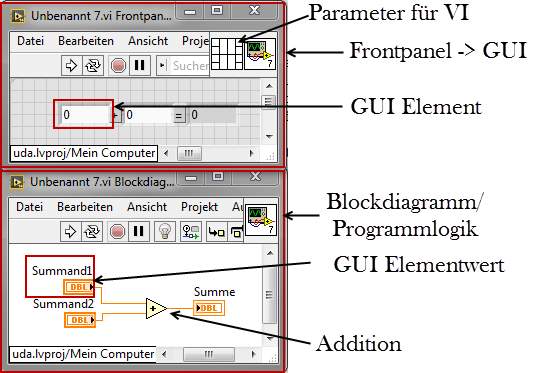
\includegraphics[width=0.6\textwidth]{LabVIEWExample}
		\caption{Beispiel LabView VI mit Beschreibung}
		\label{fig:LabViewExample}
	\end{center}
\end{wrapfigure}
LabView ist eine graphische Programiersprache, welche von National Instruments entwickelt wird. Die Funktionsweise von LabVIEW ist zudem sehr speziell es gibt Funktionsblöcke, welche Virtuelle Instrumente (VIs) bezeichnet werden. Diese VIs besitzen immer ein Frontpanel sowie ein Blockdiagramm, in welchem auch der Code zu finden ist (Siehe Figure \ref{fig:LabViewExample}). Zudem unterstützt LabVIEW seit geraumer Zeit Objektorientiertes Programmieren, dies jedoch nur unzulässig oder sehr eingeschränkt.
\newline
Wegen diesem Umstand, der mangelnden Objektorientierter Programmierfähigkeit, musste an einigen orten mit einer anderen Art und Weise angegangen werden, wie man es sich gewohnt ist. Zudem sind LabView Programme nicht sonderlich schnell, weshalb es viele Verschiedene Tasks gibt.
\newline
Eine weitere Sonderheit ist die Verknüpfung von GUIs mit dem Programm, es ist sehr stark mit dem GUI verknüpft, welches Vor- wie auch Nachteile bietet. So wird bei unserem Projekt stark mit Subpanels gearbeitet, welches die Möglichkeit liefert dynamisch GUIs von anderen VIs in das laufende Programm einzubinden.


\subsection{Software}
\subsubsection{Bestehende Software}
Im Rahmen eines Umzuges der Testabteilung, wurden die Brandräume neu gebaut. Während des Baus wurde zudem die veraltete Software, welche für die Alten Brandräume erstellt wurde. Die neu erstellte Software, welche unter dem Namen Fire Test Commander fortan nur noch FTC, wurde mit LabView erstellt. Diese Software hat schon viele Ansätze, welche für die im Rahmen dieses Projektes zu implementierendes Programm angewandt und übernommen werden können.

Der FTC bietet schon eine Struktur, um mit möglichst geringen aufwand Hardwarekomponenten hinzuzufügen (Siehe Figure \ref{fig:SystemViewFTC}). Diese Struktur, dient zudem gleich als Vorlage für die neu zu entwickelnde Software.
\begin{figure}[htbp] 
	\centering
	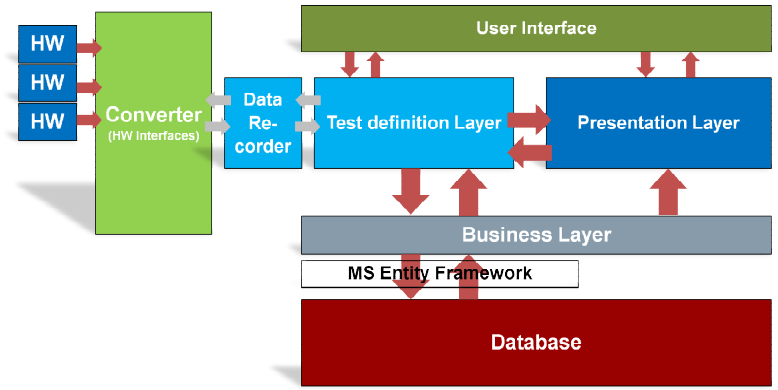
\includegraphics[width=0.5\textwidth]{SystemviewFTC}
	\caption{Systemview des Fire Test Commander}
	\label{fig:SystemViewFTC}
\end{figure}

\subsubsection{Systemgrenzen}
Da die Hardware Abstraktion komplett von der bestehenden Software übernommen werden kann, fällt diese aus dem Projekt heraus. Nur die UDA selber als eigenständige Software entwickelt. Die Abgrenzung des Systemes, kann in folgender Abbildung (Figure \ref{fig:SystemView}) nachvollzogen werden.
\begin{figure}[htbp] 
	\centering
	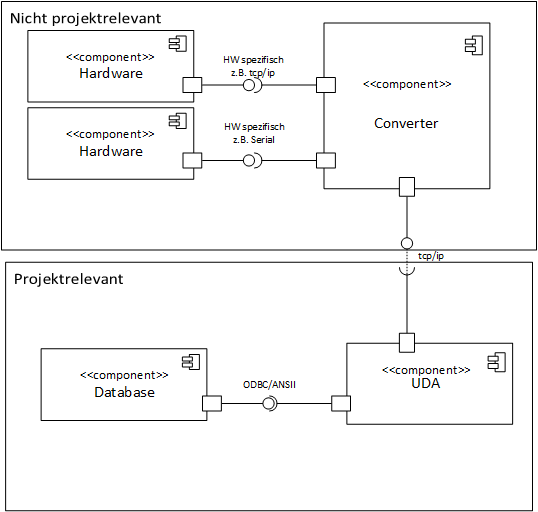
\includegraphics[width=0.35\textwidth]{Systemgrenzen}
	\caption{Systemabgrenzung der einzelnen Komponenten}
	\label{fig:SystemView}
\end{figure}

\subsubsection{Komponente UDA}
Die Softwarestruktur der FTC-Software basiert auf dem Queued Message Handler Template von National Instruments. Das Hauptprogramm (Main) besteht aus zwei parallelen Tasks
\begin{itemize}
	\item dem Event-Handler, der primär auf Eingaben vom Anwender reagiert
	\item und der Verarbeitungstask (Queued Message Handler), der die Aufträge aus seiner Message-Queue entnimmt und der Reihe nach abarbeitet.
\end{itemize}

Die Bedienoberfläche umfasst vier Subpanel-Vis. Diese werden im Hauptprogramm aufgerufen und laufen parallel zu den beiden Tasks des Hauptprogrammes. Das Frontpanel eines dieser Subpanel-Vis wird programmatisch im Subpanel des Hauptprogrammes sichtbar gemacht.  
Jedes dieser Subpanel-Vis besitzt einen eigenen Event-Handler der auf Eingaben des Anwenders reagiert. Sowohl der Event-Handler des Hauptprogrammes wie auch diejenigen der Subpanel-Vis senden Messages an die Message-Queue der Verarbeitungstask im Hauptprogramm (In der Abbildung mit grünen durchgezogenen Pfeilen dargestellt).

Aufgrund der Sonderheiten von LabView wurde die Software mit vielen verschiedenen Task ausgestattet. So ist jede GUI komponente, welche auf dem Hauptprogramm aufrufbar ist ein eigener Thread. Die Gui Komponenten werden zur entsprechenden Zeit dynamisch in der Hauptkomponente als Subkomponenten geladen. Diese Komplexe Thread Struktur wird im Folgenden Bild dargestellt.


\begin{wrapfigure}{r}{0.4\textwidth}
	\begin{center}
		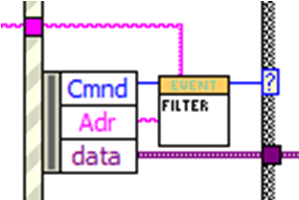
\includegraphics[width=0.3\textwidth]{filterVI}
		\caption{Aufruf des FilterVIs}
		\label{fig:filterVI}
	\end{center}
\end{wrapfigure}
Die Im Bild \ref{fig:LaufzeitansichtUDA} dargestellten Pfeile stellen die Kommunikationswege dar. Da es nicht nur eine Möglichkeit gibt mit den Threads zu kommunizieren sondern zwei. Die Erste ist mithilfe einer Queue gelöst, welche alle Threads teilen, dabei kann noch eine
Die Kommunikation vom Queue Handler zu den Event-Handlern der Subpanel-Vis des Hauptprogramms erfolgt mit User-Events (In der Abbildung \ref{fig:LaufzeitansichtUDA} mit orangen gestrichelten Pfeilen dargestellt). Die User-Events werden an alle Event-Handler gesendet (Broadcast). Mit Hilfe eines Filter-Vis (siehe Figure \ref{fig:filterVI}) kann der empfangende Event-Handler die Events aber filtern, sodass er nur Events mit der richtigen Adresse (ID) verarbeitet.

\begin{figure}[htbp] 
	\centering
	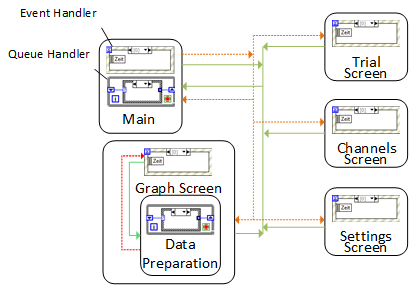
\includegraphics[width=0.9\textwidth]{Laufzeitansicht}
	\caption{Laufzeitansicht der GUI Tasks und deren Kommunikation}
	\label{fig:LaufzeitansichtUDA}
\end{figure}

\subsubsection{Data Preparation \& Recorder}

\subsection{Datenbank}
\subsubsection{Bestehende Datenbank}
Mit der implementierung der FTC Software wurde auch eine eigens dafür entwickelte Datenbank aufgebaut. Diese ist in sich enorm Komplex und sehr verstriekt, weshalb ich hier nicht viel näher auf diese eingehen kann.
\subsubsection{Datenbank}
Da wie schon erwähnt Software übernommen wird (So die gesammte Hardwareabstraktion) muss auch die Datenbank an diesen Stellen, mit einigen kleineren anpassungen, übernommen werden. Um die Funktionalität der übernommenen Komponenten zu gewährleisten wurde eine DB Schema der bisherigen Datenbank so abgespeckt (Siehe Figure \ref{fig:DBSchemaUDA}), dass Sie für die UDA brauchbar ist.
\begin{figure}[htbp] 
	\centering
	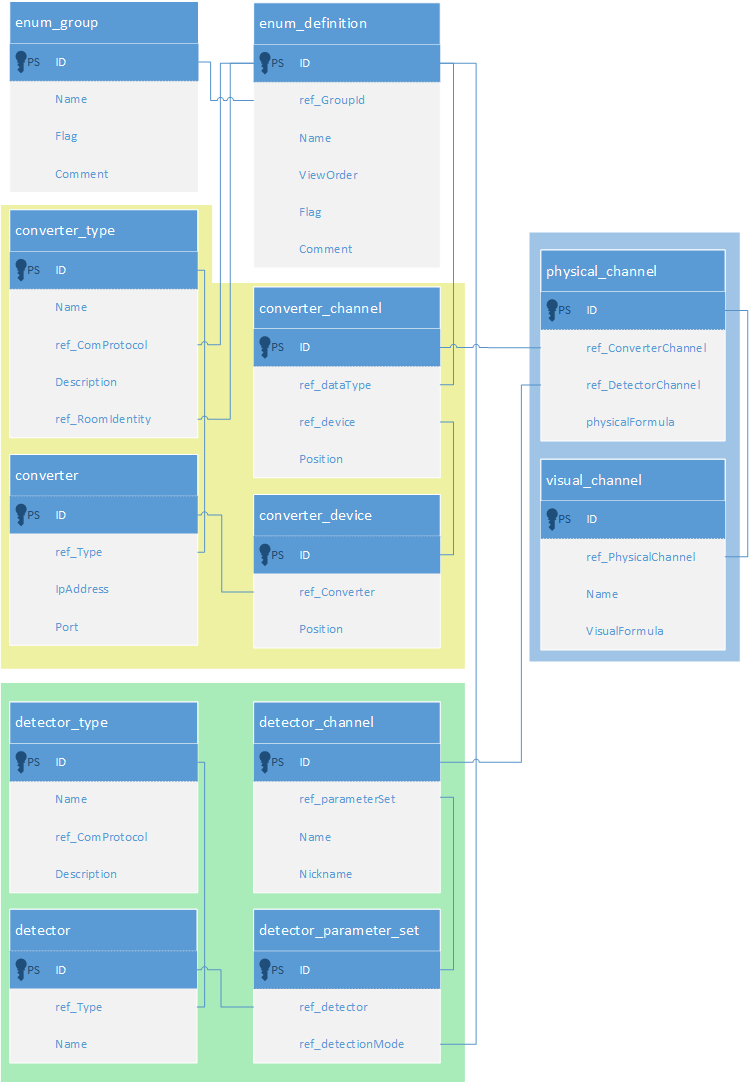
\includegraphics[width=0.4\textwidth]{DBSchemaUDA}
	\caption{Vereinfachtes DB-Schema für die UDA}
	\label{fig:DBSchemaUDA}
\end{figure}

Die Bestehende Datenbank des FTC ist sehr komplex und beinhaltet sogar eine Rechteverteilung. Da die neue Software um einiges Schlanker wird und auch nicht eine solch komplexe Struktur der Datenbank verlangt, werden nur teile der Bestehenden Datenbank entnommen, welche mit der Hardwareabstraktion zu tun hat. Dies gewährleisted, dass die Komponente, welche übernommen wird ohne Probleme weiterhin funktioniert. 
\section{Projektergebnis}
Es konnte ein Skelet einer Neuen Datenerfassungs Software erstellt werden, welche für in weiteren Schritten verbessert und erweitert wird. Die Software wurde schon nach dem ersten erfolgreichen Datenaufzeichnen Angewendet und wird im moment für 2 Testaufbauten betrieben. Sie speichert die Daten persistent und erstellt auswertbare Excel Dateien, mit denen die Testdesigner Auswertungen zu den Tests machen können.
Eine Installationsanleitung erleichtert zudem die Installation, da die Anleitung Schritt für Schritt mit Bildern erklärt wird.
Die Softwaredokumentation sowie die Bedienungsanleitung wurden in Absprache mit den Vorgesetzten im moment noch klein gehalten, da Sie zuerst das Skelett der Software wollten. Der grund für die Schnelle einführung der Software, war eine Anpassung einer UL Norm, welche dafür sorgte, dass die Melder mit einer Neuen Apparatur möglichst schon zu beginn des Projektes getestet werden sollten.

\section{Arbeitsjournal}
\begin{center}
	\begin{tabular}{p{6cm} | l | r}
		\textbf{Tätigkeit} & \textbf{Zeitraum} & \textbf{Aufwand} \\ &&\textbf{(t a 8h)}\\
		\hline Analyse der Anforderungen & W1 & 1 \\
		\hline Einarbeit in die Bestehende Software & W1 - W2 & 4 \\
		\hline Planung & W3 & 2.5 \\
		\hline SW-Design & W3-4 & 1.5 \\
		\hline DB-Modell & W4 & 1.5 \\
		\hline DB-Erstellen (Installieren und DB Modell umsetzten) & W4 - W5 & 1 \\
		\hline GUI Design & W5 & 2 \\
		\hline DB Kommunikation & W5 - W6 & 2.5 \\
		\hline Settings Screen (ini file modifikation) & W6 - W7 & 2 \\
		\hline Channels Screen (anzeige von DB info) & W7 & 1.5 \\
		\hline Graph Screen (ohne Kommunikation) & W8 - W9 & 4 \\
		\hline Recorder Implementation (Kommunikation zu Hardware Komponente) & W9 - W10 & 3.5 \\
		\hline Implementation Excel Export & W10 - W11 & 3 \\
		\hline Graph Screen inbetriebnahme mit Kommunikation & W11 - W12 & 3 \\
		\hline Fertigstellung des Software Skelettes (Zusammenführen aller Komponente) & W13 & 2 \\
		\hline Installer erstellen & W13 - W14 & 1 \\
		\hline Inbetriebnahme (Gebrauch der Software mit ankunft des neuen Aufbaus) & W14 & 3 \\
		\hline Installationsanleitung & W14 & 1 \\
		\hline SW-Dokumentation (beginn bei planung wurde jeweils ergenzt und am schluss nochmals zusammengetragen) & W14 & 0.5 \\\hhline{~--}
		& \textbf{Summe:} & \textbf{40.5} \\\hhline{~~=}
	\end{tabular}	
\end{center}
\section{Fazit}
Für mich war und ist die UDA ein enorm grosses Projekt, welches mich sicher noch ein weiters Jahr beschäftigen wird, da es noch viele features zu implementieren gilt.

Ich muss jedoch gestehen, ich habe die Arbeit unterschätzt. Es gab ja Architektonisch schon eine Software von der ich Komponenten und Teile übernehmen konnte, so stellte mir LabVIEW jedoch sehr viele hindernisse in den Weg. Bei allen Objekte, welche ich von der bestehenden Software übernehmen wollte musste ich viele Teile der Software neu implementieren, da LabVIEW viele probleme mit abhängikeiten bereitete.

Weiter hatte ich einige Schwirigkeiten, bis ich das Aufzeichnen der Daten hingekriegt habe. Hier half jedoch, dass die Hardwarekomponenten schon klar eine Schnittstelle definiert hatten. Es dauerte jedoch sehr lange bis ich eine passende lösung gefunden habe, da ich für die Integrität des Lesens, also das die Software wirklich immer in einem gewissen Zeitintervall die Daten speichert. Da ich in dieser Funktion einen eigenen Task erstellen musste und LabVIEW hier auch so seine schwächen hat.

Als Fazit für mich muss ich leider sagen, dass ich für Projekte dieser Grössenordung dringend von LabVIEW abrate. Man hat zwar schnell das Skelett des GUIs und eine gewisse Grundfunktionalität, jedoch lässt der Mangel an Wartbarkeit die Software Komplexität ins unermessliche steigen. Denn obwohl LabVIEW inzwischen OOP und unit Tests kennt, sind diese nur unzureichend brauchbar.
\section{Bestätigung Arbeitgeber}
\bibliography{literature}
\bibliographystyle{ieeetr}
\end{document}